\section{Introduction}

\begin{figure*}[t]
\centering
\begin{subfigure}{0.36\textwidth}
  \centering
  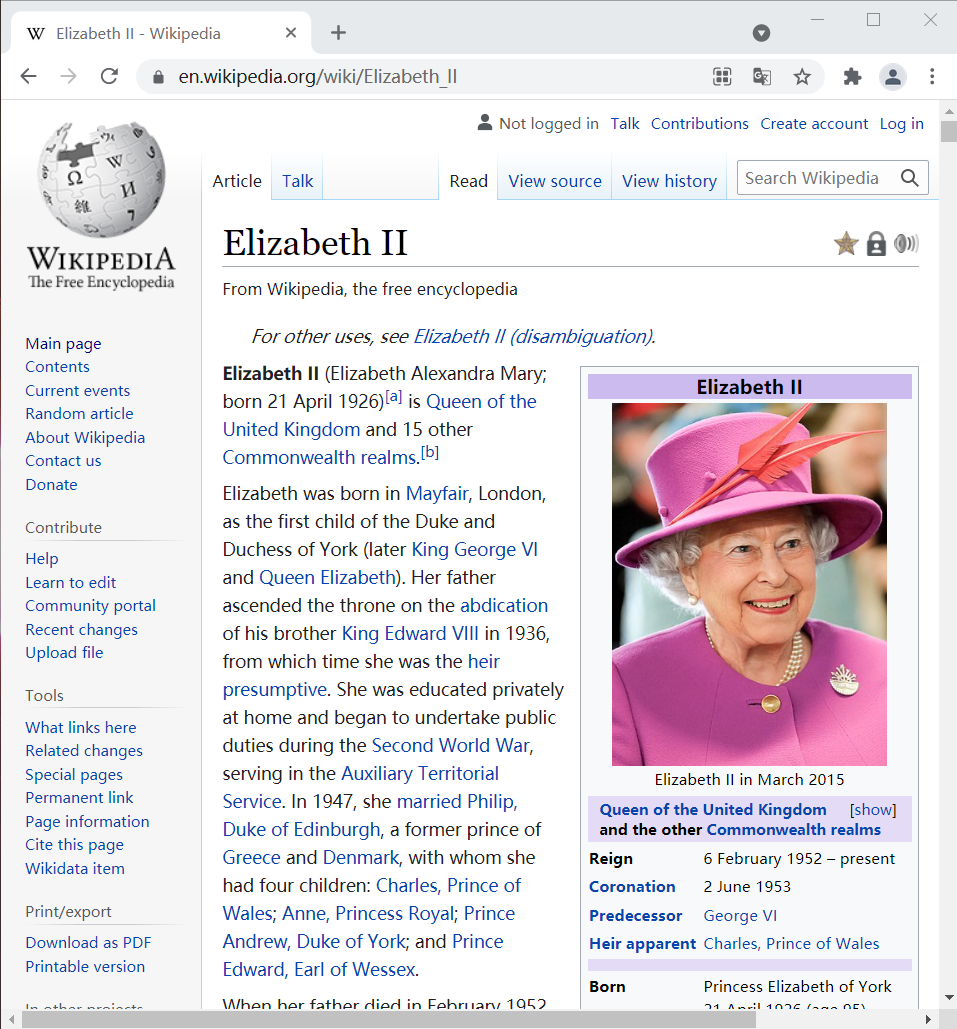
\includegraphics[width=1\textwidth]{intropage_pc}
  \caption{PC}
  \label{intropage_pc}
\end{subfigure}%
\hspace{0.25in}
\begin{subfigure}{0.3\textwidth}
  \centering
  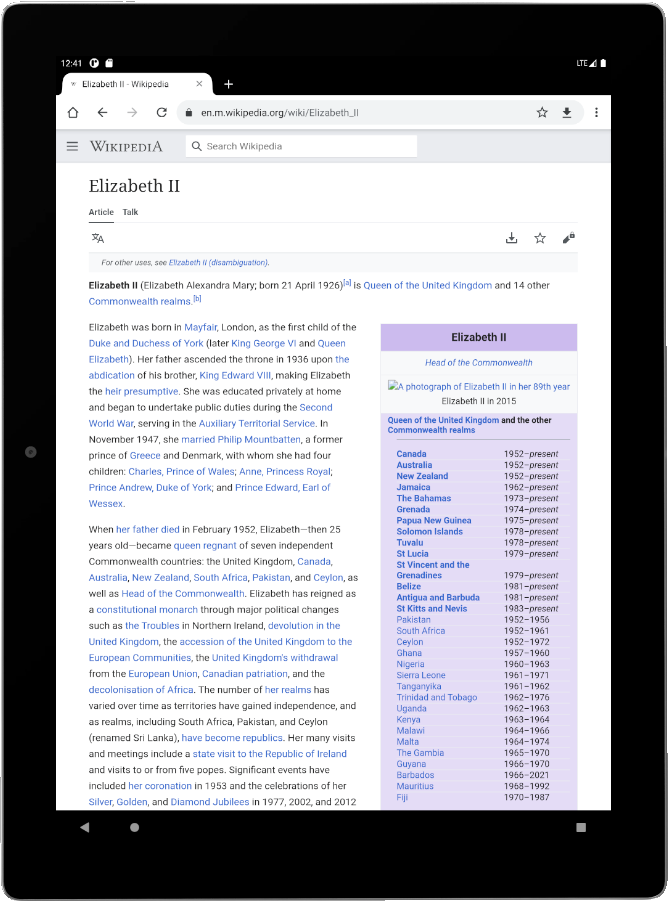
\includegraphics[width=1\textwidth]{intropage_tablet}
  \caption{Tablet}
  \label{intropage_tablet}
\end{subfigure}%
\hspace{0.25in}
\begin{subfigure}{0.2\textwidth}
  \centering
  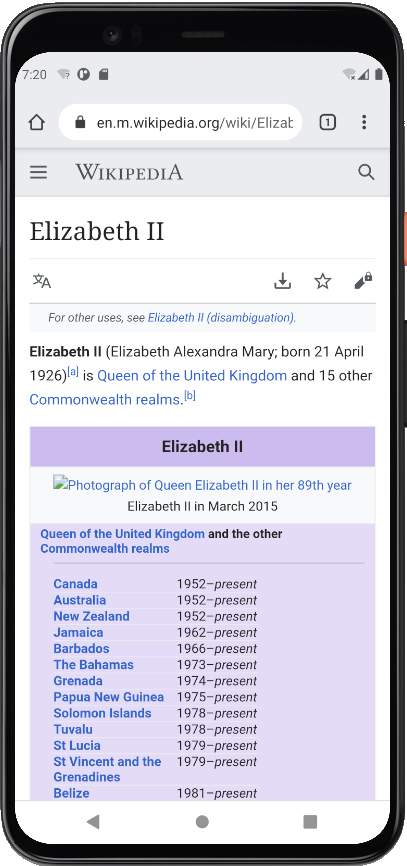
\includegraphics[width=1\textwidth]{intropage_phone}
  \caption{Android Phone}
  \label{intropage_phone}
\end{subfigure}
\caption{A sample web page rendered with different devices}
\label{intropage}
\end{figure*}

Nowadays, hyperlink texts are omnipresent on websites. However, the click popularity of these hyperlinks varies greatly. Some popular links can get clicked for million times while only a small fraction gets regularly clicked. In English Wikipedia, a previous study \cite{paranjape2016improving} stated that 66\% links were not clicked even a single time in March 2015 and that only around 4\% of all the existing links are clicked by visitors more than 10 times within a month \cite{dimitrov2017makes}. Such imbalance may imply that many hyperlinks are not meeting the information need of users, or some potentially valuable pages are being ignored. 

To tackle this issue, we need to have a clear idea of the factors affecting click popularity. We study this problem by modeling the task of click popularity prediction with the potential factors. We assume that all of the entity mentions have been correctly recognized, disambiguated, and linked. Given that the click popularity of a hyperlink can be reflected by the number of views the article receives, we consider predicting Click Through Rate (CTR). Since the number of hyperlinks can vary greatly between different web pages, we formulate our problem as ranking to eliminate its impact. To be specific, we predict the relative CTR rank of hypertext links on a certain article instead of the absolute CTR value.

Many factors are contributing to the hypertext link click popularity.  Previous works mainly focus on textual and graph-based features \cite{thruesen2016link, yamada2018linkify}. However, they neglected the significant impact of visual factors. In fact, a large share of user clicks comes from links in the lead section or the infobox \cite{lamprecht2017structure}. Links in these two sections are more eye-catching and thus get more attention. Therefore, we are particularly interested in the effect of visual factors in this work. 

Understanding what visual factors can affect users' click behavior can be instructive to the amelioration of website structure organization. For example, we can improve the browsing experience with better-organized hyperlink placement. Figure \ref{intropage} presents a popular Wikipedia webpage named \emph{Elizabeth II} \footnote{https://en.wikipedia.org/wiki/Elizabeth\_II}. Even such a carefully-edited webpage may not have been organized optimally in terms of the efficiency in seeking important information. Suppose that a user visits this page on PC and wishes to obtain some relevant information about her interpersonal relationship. The key hyperlinks like \emph{Prince Philip, Duke of Edinburgh} and \emph{Anne, Princess Royal} are hard to be spotted at first glance. Instead, two relatively trivial links (\emph{Queen of the United Kingdom} and \emph{Commonwealth realms}) have appeared twice in the most exposed positions. For better structure organization, we can reinforce some strongly related links by simply changing their visual appearances, for example, by locating them on the top of the page, so that users can obtain relevant information with ease. 

In limited work considering visual features \cite{dimitrov2016visual, dimitrov2017makes}, the authors render HTML pages on PC under $1920 \times 1080$ resolution and then obtain the coordinate positions of hyperlinks as a type of feature. As a result, the authors found out that people preferred to click on those links that are located at the top of the screen in the lead section, or on the left side of the body. Although this work showed the relevance between click popularity and visual features, this approach has three drawbacks. 

First, the computation burden is heavy. The visual features cannot be obtained until the whole HTML page has been completely rendered. Second, these features are specific to Wikipedia. For example, whether or not a hyperlink is located in the infobox was considered as a feature. It is impossible to apply this feature to other domains. Third, it is not reasonable to assume that all users browse web pages exactly under the same scenario. As is shown in Figure \ref{intropage}, even the same web page can be rendered quite differently under different settings. Much less content can be rendered on screen for the Android phone than PC and tablet. Many hypertext links on the PC and tablet remain unspotted on the Android phone unless the readers scroll down the explorer. Besides, the coordinate positions of these hyperlinks are also different. If people tend to click hyperlinks located in the left part of the screen, the prediction of click popularity could be quite different between these three devices.

Therefore, visual features should be generalizable to other domains and independent of specific settings like devices and resolutions. In this work, we propose five visual features for click popularity prediction: \emph{section position}, \emph{distance to the nearest picture}, \emph{distance to the nearest subtitle}, \emph{distance to nearest table} and \emph{within table}. All five visual features do not require rendering web pages. More importantly, the proposed visual features can be further combined with other sorts of feature groups like textual and graph-based features \cite{thruesen2016link, dimitrov2017makes} to improve accuracy for the Learning to Rank model.

To examine the effectiveness of different features, we conduct two sets of controlled experiments: \emph{source link} and \emph{target link}. In \emph{source link}, we are going to rank incoming hyperlinks to a certain article. Similarly, for \emph{target link}, we will rank the outgoing hyperlinks from an article. Such two-direction experiments can help us take the effect of both source/target page into consideration, so as to doubly validate the importance of the features alone. To reach a generalizable conclusion, we tested under ten different domains (People, Mass media, Culture, etc). As we focus on the impact of visual properties on click popularity, we also conduct experiments ruling out other irrelevant factors. According to the experimental result, the visual features are helpful for hyperlink click popularity prediction. The performance of the Learning to Rank model significantly gets improved after adding visual features.

Besides, we compare our proposed visual features with the previous ones that require rendering \cite{dimitrov2017makes}. We consider PC and mobile phone setting \footnote{The share of tablet devices worldwide is very small https://gs.statcounter.com/platform-market-share/desktop-mobile-tablet}. For the PC setting, we tested three most widely-used resolutions ($1366\times768$, $1536\times864$ and $1920\times1080$) \footnote{https://gs.statcounter.com/screen-resolution-stats/desktop/worldwide}. As for the mobile phone setting, we tried mobile devices from the four most popular brands: Samsung, Apple, Xiaomi and Huawei \footnote{https://gs.statcounter.com/vendor-market-share/mobile/worldwide}. Furthermore, we analyze the impact of each visual feature through ablation tests and draw two conclusions. First, every visual feature we have proposed is helpful. Second, two visual features named \emph{section position} and \emph{within table} are relatively more important.

To sum up, the main contributions of this paper are listed as the following:

\begin{itemize}

    \item First, we study hyperlink click popularity prediction and propose five visual features. All visual features are render-agnostic, meaning that they are independent of devices and resolutions, and can be computed easily without rendering. Besides, our proposed visual features are orthogonal to all the other types of features, so that they can be combined with any other types of features (like textual features and graph-based) to improve accuracy for this task.

    \item Second, we validate the effectiveness of our proposed visual features. With these features, the performance of the Learning to Rank model gets significantly improved, showing consistent improvement across ten different domains. We compare our proposed visual features with the previous ones that require rendering \cite{dimitrov2017makes} under both PC and mobile phone settings. As a result, our proposed visual features can achieve higher performance, which suggests that the proposed render-agnostic visual features can adapt better to practical scenarios with various resolution settings.

    \item Third, we further conduct ablation tests to quantitively analyze the impact of each visual feature. The results indicate that every visual feature we proposed is helpful in this task. More importantly, we find that two visual features: \emph{section position} and \emph{within table} are relatively more important.

\end{itemize}
